\documentclass[11pt]{article}

\usepackage{sectsty}
\usepackage{graphicx}
\usepackage{titlepic}

% Margins
\topmargin=-0.45in
\evensidemargin=0in
\oddsidemargin=0in
\textwidth=6.5in
\textheight=9.0in
\headsep=0.25in

\title{ EEM076 Lab1 }
\author{ Albin Boklund, Samuel Runmark Thunell }
\date{\today}

\pagenumbering{gobble}

\begin{document}
\maketitle

\pagebreak

%--TASK1--

\section{\bf{Measuring currents}}

\subsection[25pt]{\bf{Calculations}}

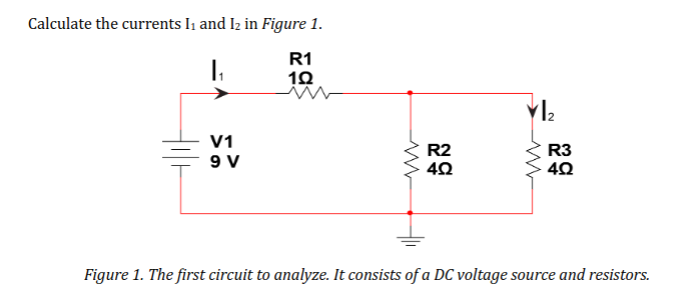
\includegraphics[width=\linewidth]{1.1 calculation.png}


\noindent
insert equation here

\subsection[25pt]{\bf{Circuit design}}

\noindent
\\
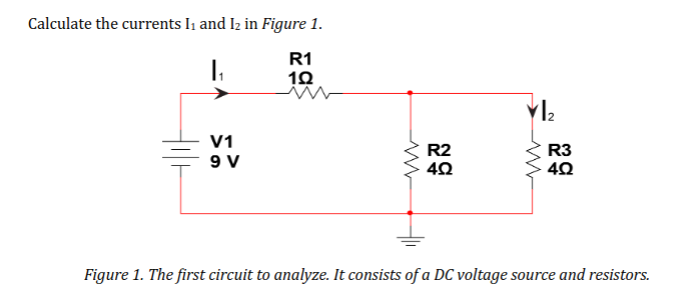
\includegraphics[width=\linewidth]{1.1 calculation.png}

insert maybe description here

\subsection[25pt]{\bf{Circuit design}}

\noindent
\\
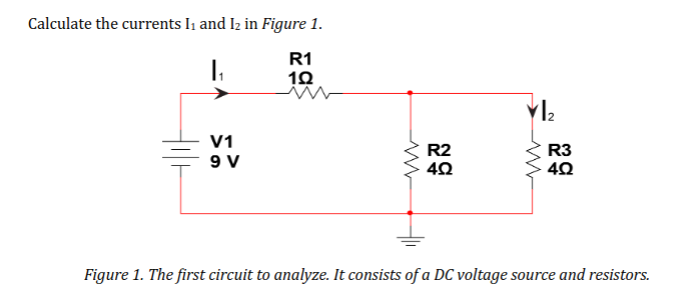
\includegraphics[width=\linewidth]{1.1 calculation.png}

insert analasys here




%--TASK2--
\section{\bf{Mesh analasys}}

\subsection[25pt]{\bf{Calculations}}

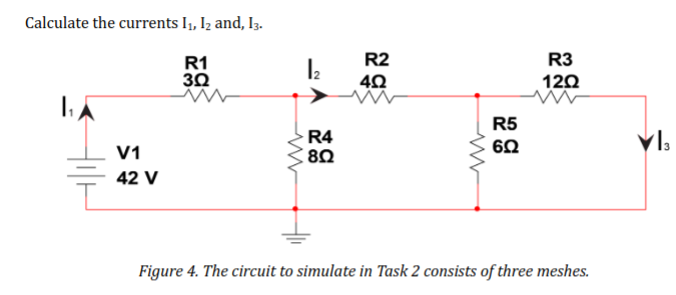
\includegraphics[width=\linewidth]{2.1 calculations.png}


\noindent
insert equation here

\subsection[25pt]{\bf{Circuit design}}

\noindent
\\
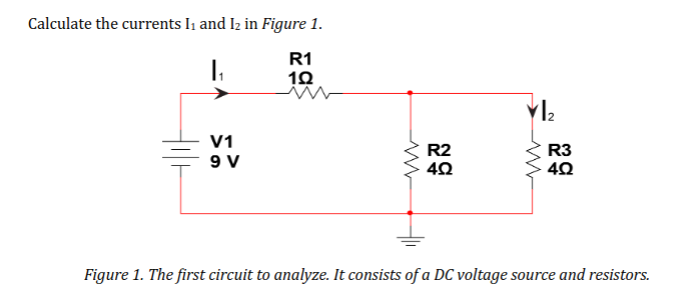
\includegraphics[width=\linewidth]{1.1 calculation.png}

insert maybe description here

\subsection[25pt]{\bf{Simulation}}

\noindent
\\
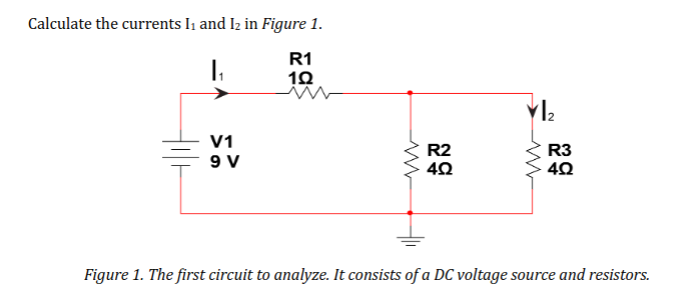
\includegraphics[width=\linewidth]{1.1 calculation.png}

insert analasys here


%--TASK3--
\section{\bf{The Superposition Principle}}

\subsection[25pt]{\bf{Calculations}}

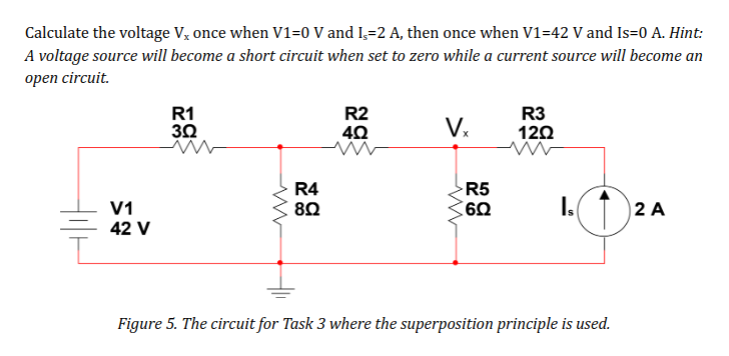
\includegraphics[width=\linewidth]{3.1 calculations.png}


\noindent
insert equation here

\subsection[25pt]{\bf{Circuit design}}

\noindent
\\
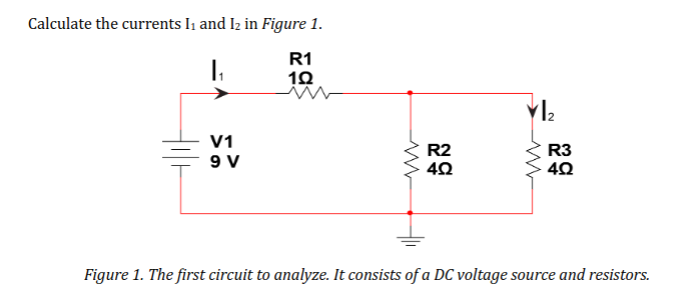
\includegraphics[width=\linewidth]{1.1 calculation.png}

insert maybe description here

\subsection[25pt]{\bf{Simulation}}

\noindent
\\
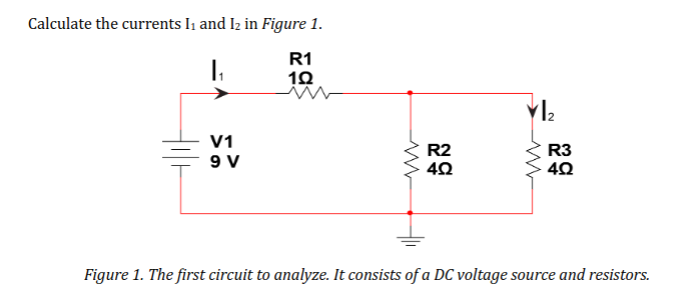
\includegraphics[width=\linewidth]{1.1 calculation.png}

insert analasys here


%--TASK4--
\section{\bf{Input and Output impedance}}

\subsection[25pt]{\bf{Calculations}}

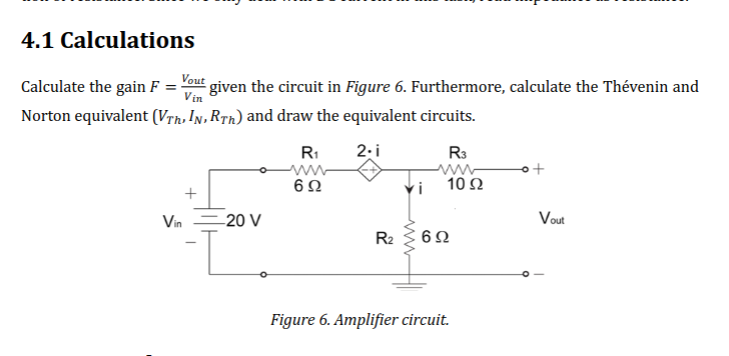
\includegraphics[width=\linewidth]{4.1 calculations.png}


\noindent
insert equation here

\subsection[25pt]{\bf{Circuit design}}

\noindent
\\
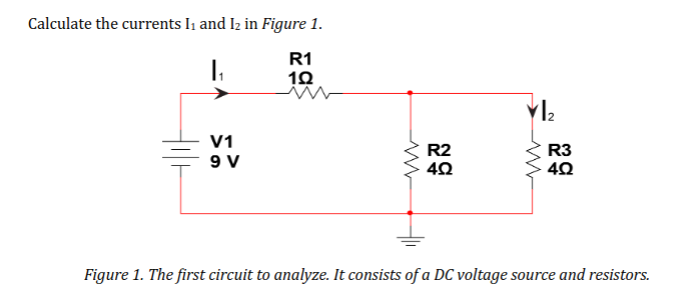
\includegraphics[width=\linewidth]{1.1 calculation.png}

insert maybe description here

\subsection[25pt]{\bf{Simulation}}

\noindent
\\
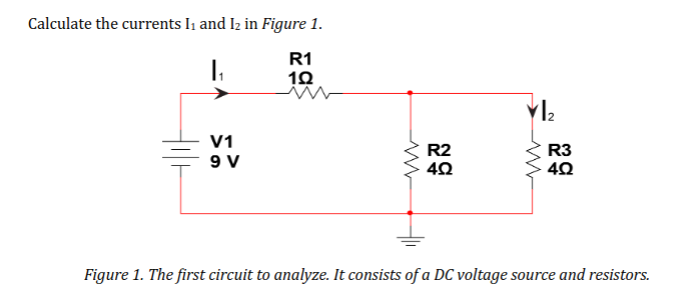
\includegraphics[width=\linewidth]{1.1 calculation.png}

insert analasys here


%--TASK5--
\section{\bf{Maximal power from a voltage source}}

\subsection[25pt]{\bf{Calculations}}

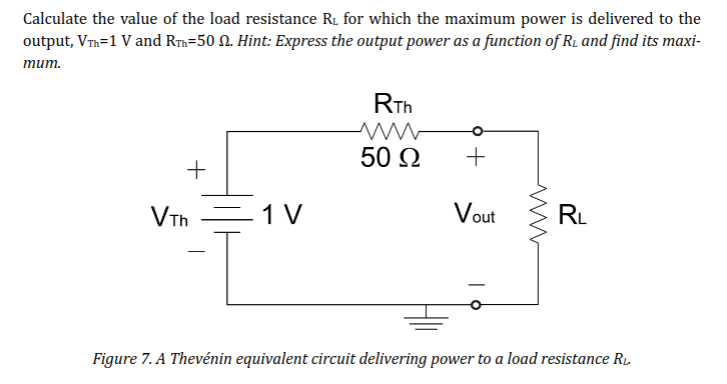
\includegraphics[width=\linewidth]{5.1 calculations.png}


\noindent
insert equation here

\subsection[25pt]{\bf{Circuit design}}

\noindent
\\
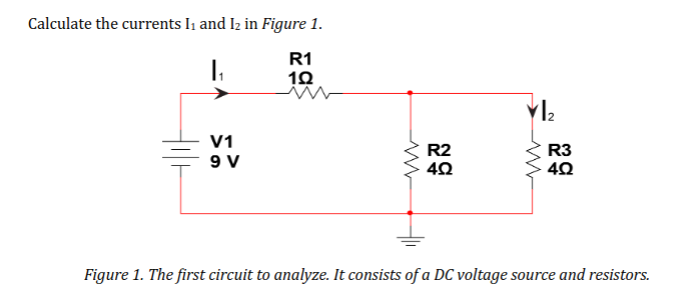
\includegraphics[width=\linewidth]{1.1 calculation.png}

insert maybe description here

\subsection[25pt]{\bf{Simulation}}

\noindent
\\
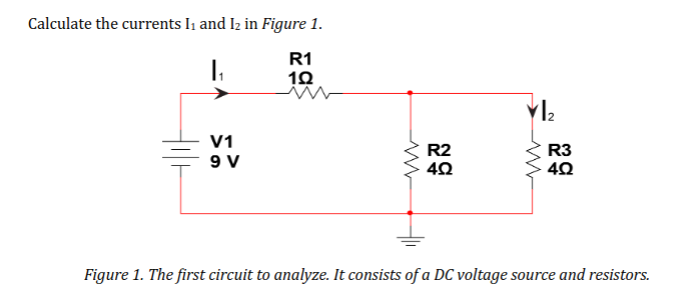
\includegraphics[width=\linewidth]{1.1 calculation.png}

insert analasys here


%--TASK6--
\section{\bf{Maximum power from a current source}}

\subsection[25pt]{\bf{Calculations}}

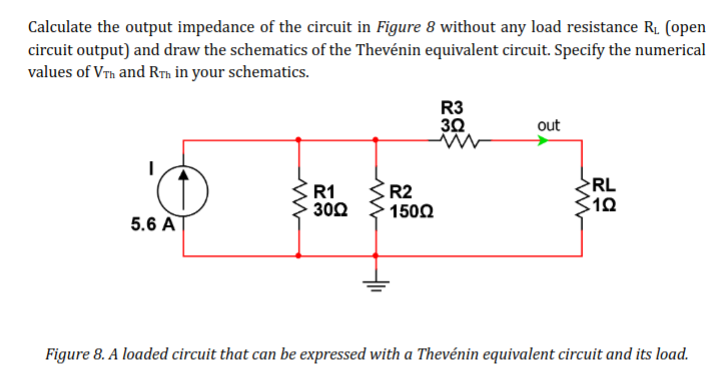
\includegraphics[width=\linewidth]{6.1 calculations.png}


\noindent
insert equation here

\subsection[25pt]{\bf{Circuit design}}

\noindent
\\
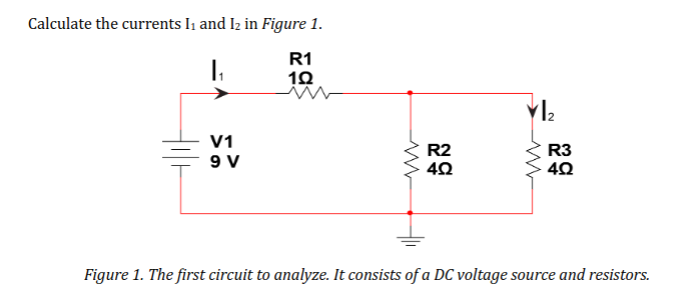
\includegraphics[width=\linewidth]{1.1 calculation.png}

insert maybe description here

\subsection[25pt]{\bf{Simulation}}

\noindent
\\
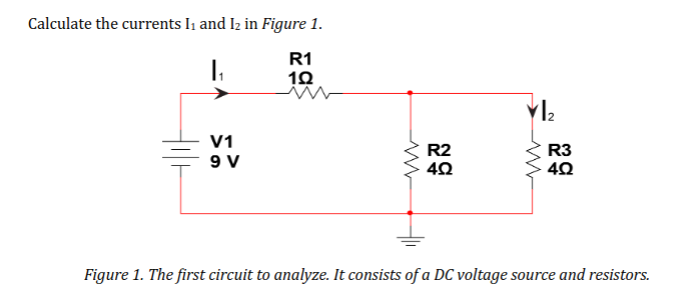
\includegraphics[width=\linewidth]{1.1 calculation.png}

insert analasys here


\end{document}